\documentclass{ximera}

%\newtheorem{theorem}{Theorem}%[section] % reset theorem numbering for each section
%\newtheorem*{theorem*}{Theorem}%[section] % reset theorem numbering for each section
\newtheorem{prop}[theorem]{Proposition}
\newtheorem{lem}[theorem]{Lemma}
\newtheorem{ex}{Example}


\title{Quadratic reciprocity}  
\begin{document}  
\begin{abstract}  
We finally prove quadratic reciprocity!\end{abstract}  
\maketitle  

\begin{theorem}[Restatement of quadratic reciprocity]
 Let $p$ and $a$ be odd primes with $p\neq q$. Then \[\left(\frac{p}{q}\right)\left(\frac{q}{p}\right)=(-1)^{\frac{p-1}{2}\frac{q-1}{2}}.\]
\end{theorem}

\begin{definition}
 A \emph{lattice point} is a point $(x,y)\in\mathbb{R}^2$ where $x,y\in\mathbb{Z}$. We can write this as $(x,y)\in\mathbb{Z}^2$.
\end{definition}

%\begin{proof}[Example 1]
%We will use  $p=7$ and $q=5$ as an example:
%
% The participation assignment is to show that there are $\frac{(p-1)}{2}\frac{(q-1}{2}$ lattice points in the rectangle $OABC$ (including those on the lines $AB$ and $BC$, but not $OA$ or $OC$). 
%
%Now, we are going to show that there are $N_1$ lattice points in the triangle $OPC$ (not including $OC$) and $N_2$ lattice points in in $OAM$ (not including $OA$), where $N_1$ and $N_2$ 
%\end{proof}
\begin{proof}
 Without loss of generality, assume that $p>q$. We draw the rectangle $O=(0,0), A=\left(\frac{p-1}{2},0\right), B=\left(\frac{p-1}{2},\frac{q-1}{2}\right),$ and $C=\left(0,\frac{q-1}{2}\right)$, like in the graphic below:

\begin{image}
 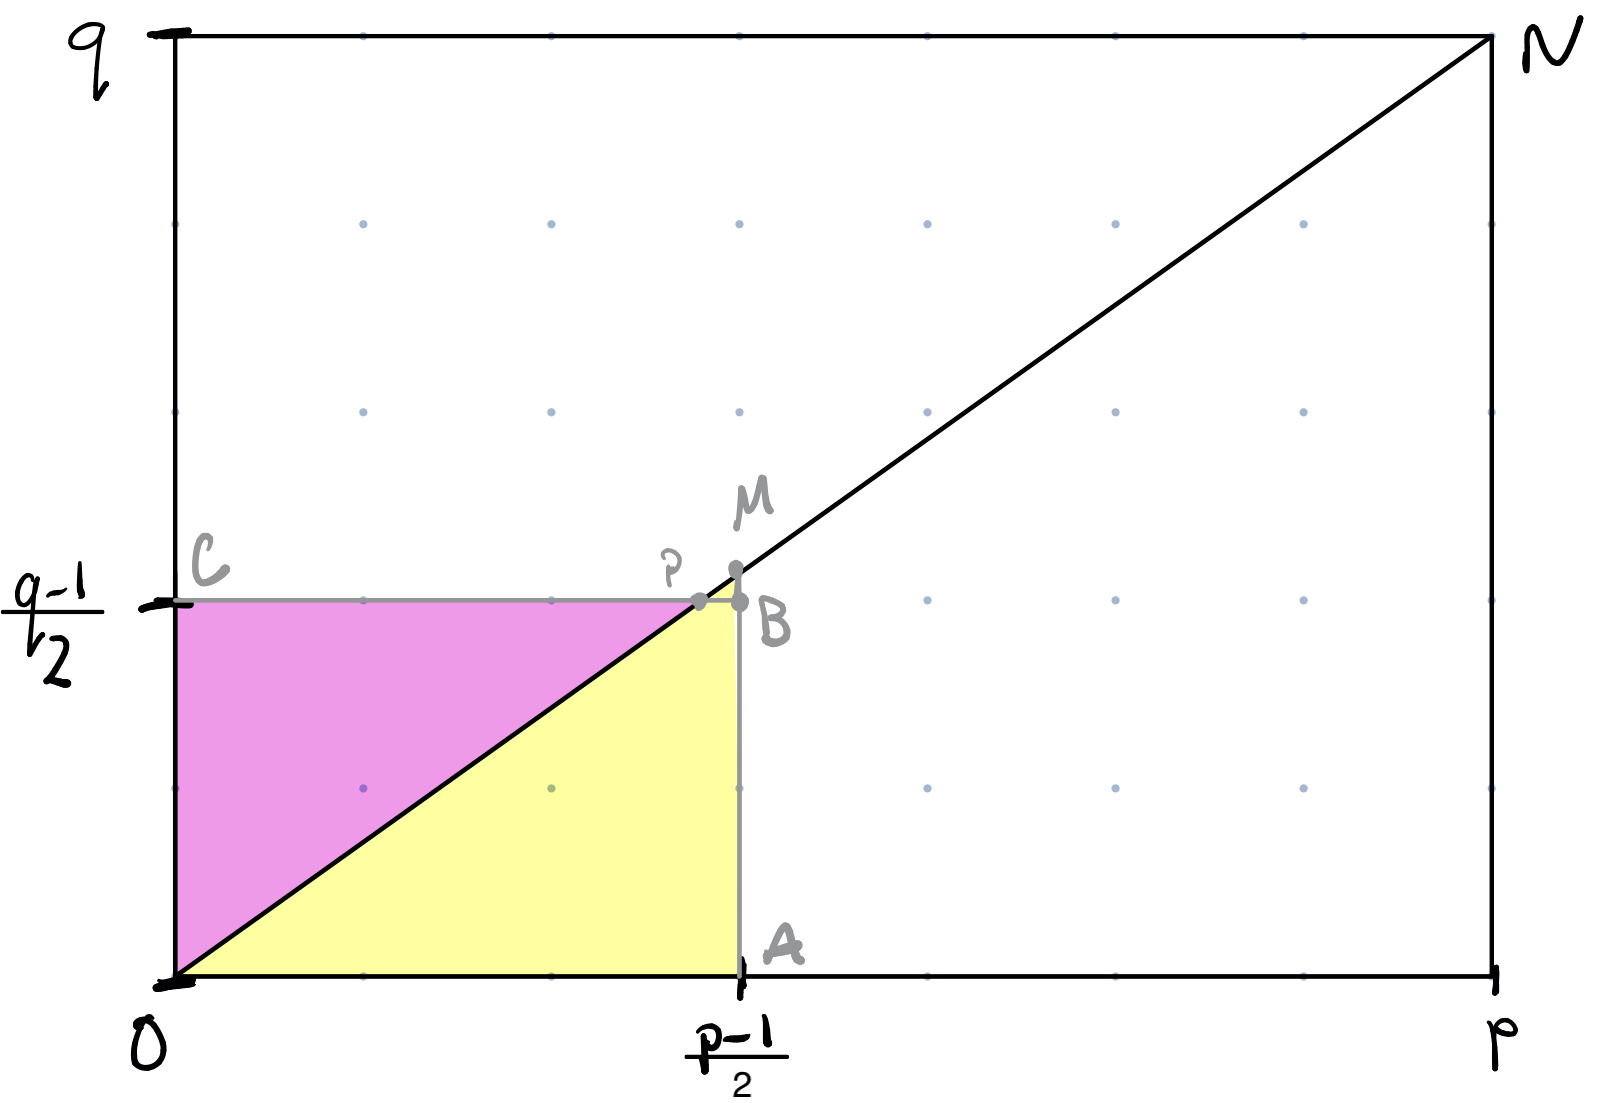
\includegraphics{lattice.jpg}
\end{image}

The participation assignment is to count the lattice points in the rectangle $OABC$ outlined in grey, including those on the lines $AB$ and $BC$, but not those on $OA$ or $OC$. 

In order to count these lattice points another way, we are going to show that there are $N_1$ lattice points in the triangle $OPC$ not including $OC$(pink)  and $N_2$ lattice points in in $OAM$ not including $OA$ (yellow), thus the total number of lattice points is $N_1+N_2$. We will find that $N_1=\sum_{j=1}^{\frac{q-1}{2}}\left\lfloor\frac{jp}{q}\right\rfloor$ and $N_2=\sum_{j=1}^{\frac{-1}{2}}\left\lfloor\frac{jq}{p}\right\rfloor$. Thus, by the previous lemma, $\left\lfloor\frac{p}{q}\right\rfloor=(-1)^{N_1}$ and $\left\lfloor\frac{q}{p}\right\rfloor=(-1)^{N_2}$, which will let us finish the proof. 

We will do an examples first:

\begin{ex}
 We look at the example above with $p=7$ and $q=5$.  
\begin{enumerate}[label=\alph*)]
 \item The line $ON$ has slope $\answer{\frac{5}{7}}
 $. Since $p$ and $q$ are distinct primes, there are no lattice points on $ON$ except the endpoints. 
 \item The $x$-coordinate of $M$ is $\answer{3}
 $, $y$-coordinate of $M$ is $\answer{\frac{15}{7}}
 $.
 \item The $y$-coordinate of $M$ lies between two consecutive integers $\answer{2}
 $ and $\answer{3}
 .$ 
\end{enumerate}

Thus, the triangle $PMB$ has no lattice points except possibly those on $PB$. We can then count the number of lattice points in $OABC$ by adding the number of lattice points in $OCP$ to those in $OAM$.

To find $N_1$, the number of lattice points in $OPC$, not including those on $OC$, we count how many lattice points on the line $y=j$ are to the left of $ON$ for $j=1,2,\dots,\frac{q-1}{2}$ (in our case, this is only $j=1,2$.) Another was of saying this is for each $j$, we want the number of nonnegative integers less than 
\begin{multipleChoice}
 \choice[correct] {$\frac{7j}{5}$}
 \choice {$\frac{5j}{7}$}
\end{multipleChoice}

 Thus, we have for each $j$, there are 
 \begin{multipleChoice}
 \choice[correct] {$\left\lfloor\frac{7j}{5}\right\rfloor$}
 \choice {$\left\lfloor\frac{5j}{7}\right\rfloor$}
\end{multipleChoice}
 
lattice points in $OPC$. Then $N_1=$
 \begin{multipleChoice}
 \choice[correct] {$\sum_{j=1}^{2
}\left\lfloor\frac{7j}{5}\right\rfloor$}
 \choice {$\sum_{j=1}^{2
}\left\lfloor\frac{5j}{7}\right\rfloor$}
\end{multipleChoice}

To find $N_2$, we use a similar counting method on $OAM$. Now, we count the lattice points on $x=j$ for $j=1,2,\dots,\frac{p-1}{2}$. Thus, for each $j$, we want the number of nonnegative integers less than \begin{multipleChoice}
 \choice{$\frac{7j}{5}$}
 \choice[correct]  {$\frac{5j}{7}$}
\end{multipleChoice}
 Thus, we have for each $j$, there are  \begin{multipleChoice}
 \choice{$\left\lfloor\frac{7j}{5}\right\rfloor$}
 \choice[correct] {$\left\lfloor\frac{5j}{7}\right\rfloor$}
\end{multipleChoice}l
attice points in $OPC$. Then $N_2=$
 \begin{multipleChoice}
 \choice[correct] {$\sum_{j=1}^{3
}\left\lfloor\frac{7j}{5}\right\rfloor$}
 \choice {$\sum_{j=1}^{3
}\left\lfloor\frac{5j}{7}\right\rfloor$}
\end{multipleChoice}

 \end{ex}
 
%\begin{ex}
%We look at the example with $p=11$ and $q=7$.  
%
% 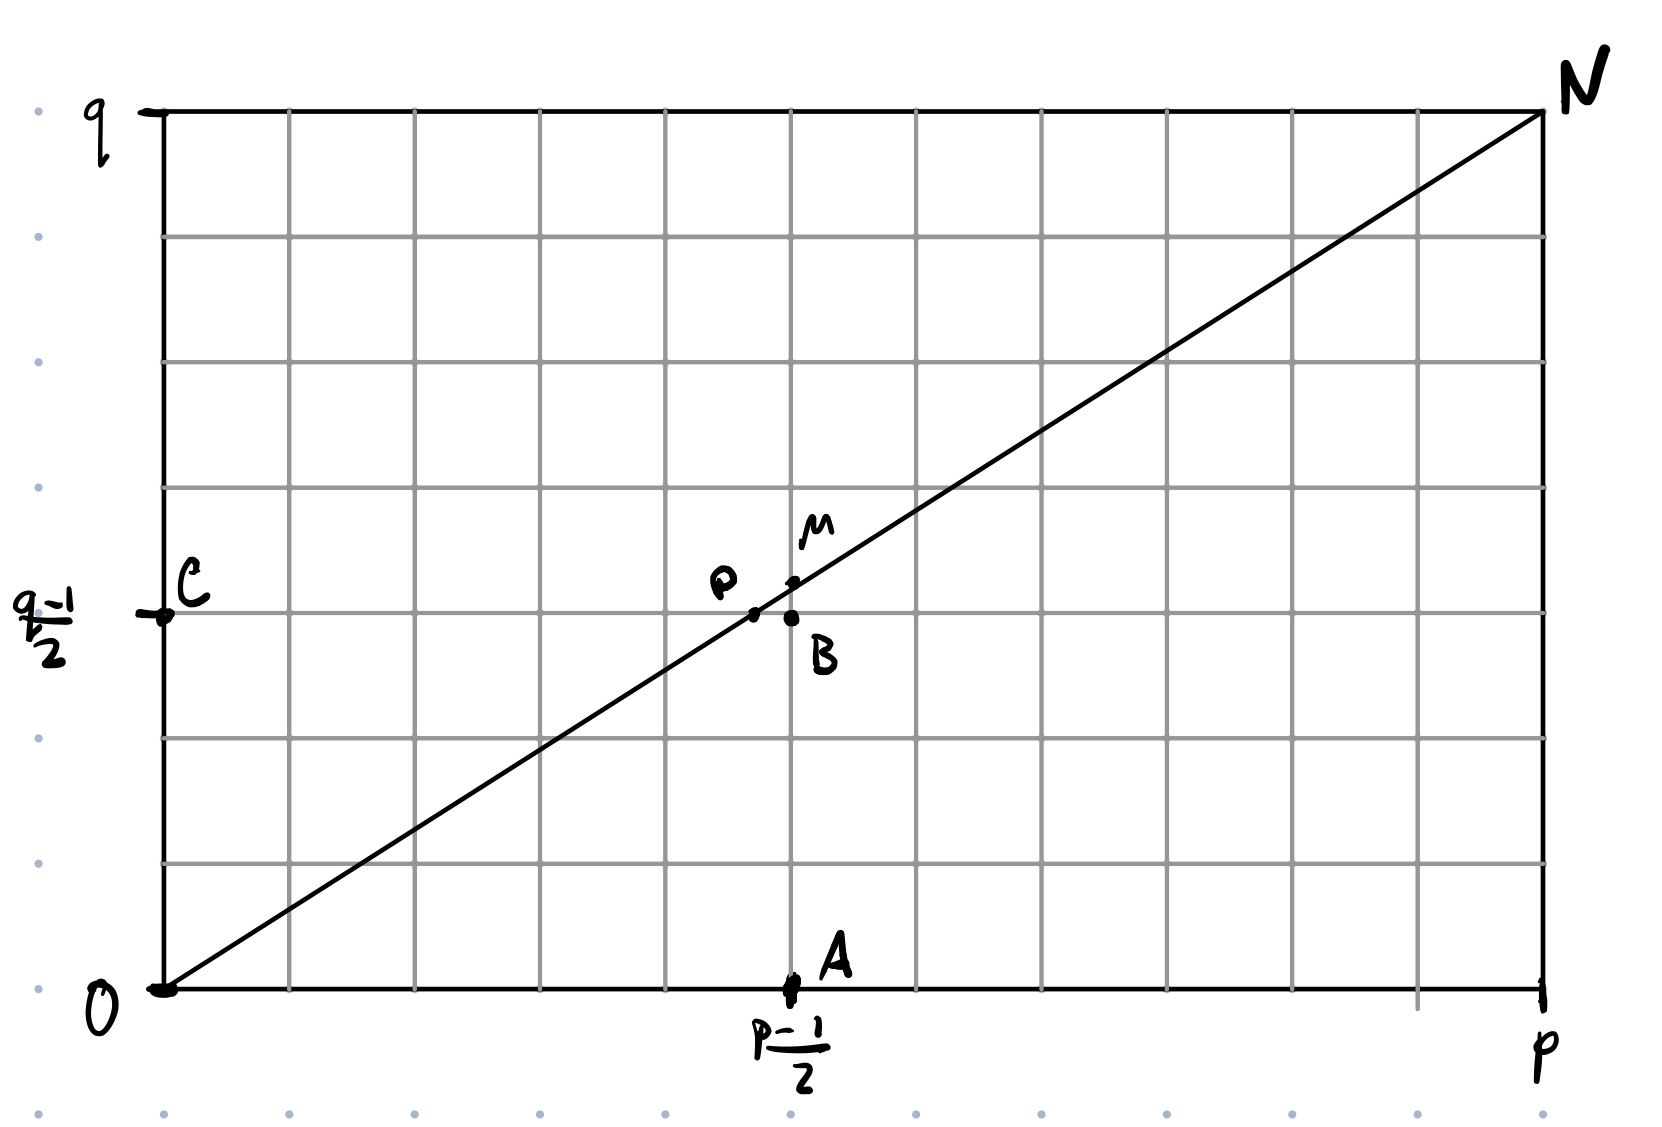
\includegraphics[width=\textwidth]{latticepoints}
%\begin{enumerate}[label=\alph*)]
% \item The line $ON$ has slope $\answer{\frac{7}{11}}
% $. Since $p$ and $q$ are distinct primes, there are no lattice points on $ON$ except the endpoints. We can represent $ON$ 
% \item The $x$-coordinate of $M$ is $\answer{5}
% $, $y$-coordinate of $M$ is $\answer{\frac{35}{11}}
% $.
% \item The $y$-coordinate of $M$ lies between two consecutive integers $\answer{3}
% $ and $\answer{4}
% .$ 
%\end{enumerate}
%
%Thus, the triangle $PMB$ has no lattice points except possibly those on $PB$. We can then count the number of lattice points in $OABC$ by adding the number of lattice points in $OCP$ to those in $OAM$.
%
%To find $N_1$, the number of lattice points in $OPC$, not including those on $OC$, we count how many lattice points on the line $y=j$ are to the left of $ON$ for $j=1,2,\dots,\frac{q-1}{2}$. Another was of saying this is for each $j$, we want the number of nonnegative integers less than $j\answer{\frac{11}{7}}
%$. Thus, we have for each $j$, there are $\left\lfloor j*\answer{\frac{11}{7}}
%\right\rfloor$ lattice points in $OPC$. Then \[N_1=\sum_{j=1}^{\answer{3}
%}\left\lfloor j*\answer{\frac{11}{7}}
%\right\rfloor.\]
%
%To find $N_2$, we use a similar counting method on $OAM$. Now, we count the lattice points on $x=j$ for $j=1,2,\dots,\frac{p-1}{2}$. Thus, for each $j$, we want the number of nonnegative integers less than $j*\answer{\frac{7}{11}}
%$. Thus, we have for each $j$, there are $\left\lfloor j*\answer{\frac{7}{11}}
%\right\rfloor$ lattice points in $OPC$. Then \[N_2=\sum_{j=1}^{\answer{5}
%}\left\lfloor j*\answer{\frac{7}{11}}
%\right\rfloor.\]
%\end{ex}

Now we generalize this idea to any odd primes $p$ and $q$ with $p>q$.
\begin{enumerate}[label=\alph*)]
 \item The line $ON$ has slope $\frac{q}{p} $. Since $p$ and $q$ are distinct primes, there are no lattice points on $ON$ except the endpoints. 
  \item The $x$-coordinate of $M$ is $\frac{p-1}{2} $, $y$-coordinate of $M$ is $\frac{(p-1)}{2}\frac{q}{p}=\frac{q}{2}-\frac{q}{2p}$.
 \item The $y$-coordinate of $M$ lies between two consecutive integers $\frac{q-1}{2}$ and $\frac{q+1}{2}$, since 
\begin{align*}
 \frac{q-1}{2}&=\frac{q}{2}-\frac{1}{2}<\frac{q}{2}-\frac{q}{2p}<\frac{q}{2}<\frac{q+1}{2}
\end{align*}
\end{enumerate}

Thus, the triangle $PMB$ has no lattice points except possibly those on $PB$. We can then count the number of lattice points in $OABC$ by adding the number of lattice points in $OCP$ to those in $OAM$.

To find $N_1$, the number of lattice points in $OPC$, not including those on $OC$, we count how many lattice points on the line $y=j$ are to the left of $ON$ for $j=1,2,\dots,\frac{q-1}{2}$. Another was of saying this is for each $j$, we want the number of nonnegative integers less than \begin{multipleChoice}
 \choice[correct] {$\frac{jp}{q}$}
 \choice {$\frac{jq}{p}$}
\end{multipleChoice} 

Thus, we have for each $j$, there are 
\begin{multipleChoice}
 \choice[correct] {$\left\lfloor\frac{jp}{q}\right\rfloor$}
 \choice {$\left\lfloor\frac{jq}{p}\right\rfloor$}
\end{multipleChoice}
 
lattice points in $OPC$. Then $N_1=$
 \begin{multipleChoice}
 \choice[correct] {$\sum_{j=1}^{2
}\left\lfloor\frac{jp}{q}\right\rfloor$}
 \choice {$\sum_{j=1}^{2
}\left\lfloor\frac{jq}{p}\right\rfloor$}
\end{multipleChoice}

To find $N_2$, we use a similar counting method on $OAM$. Now, we count the lattice points on $x=j$ for $j=1,2,\dots,\frac{p-1}{2}$. Thus, for each $j$, we want the number of nonnegative integers less than  \begin{multipleChoice}
 \choice {$\frac{jp}{q}$}
 \choice[correct] {$\frac{jq}{p}$}
\end{multipleChoice} Thus, we have for each $j$, there are \begin{multipleChoice}
 \choice{$\left\lfloor\frac{jp}{q}\right\rfloor$}
 \choice[correct]  {$\left\lfloor\frac{jq}{p}\right\rfloor$}
\end{multipleChoice}
lattice points in $OPC$. Then $N_2= $\begin{multipleChoice}
 \choice {$\sum_{j=1}^{2
}\left\lfloor\frac{jp}{q}\right\rfloor$}
 \choice[correct] {$\sum_{j=1}^{2
}\left\lfloor\frac{jq}{p}\right\rfloor$}
\end{multipleChoice}
From the previous Lemma, $\left(\frac{p}{q}\right)=(-1)^{N_1}$ and $\left(\frac{q}{p}\right)=(-1)^{N_2}$. Thus, 
\begin{align*}
 \left(\frac{p}{q}\right)\left(\frac{p}{q}\right)&=(-1)^{N_1} (-1)^{N_2} \\
 &=(-1)^{N_1+N_2}\\
&=(-1)^{\frac{p-1}{2}\frac{q-1}{2}}
\end{align*}
with the result from the participation assignment.
\end{proof}

Quadratic reciprocity means that determining all quadratic residues (perfect squares) modulo an odd prime is a finite problem. In terms of Legendre symbol, this is finding all $a$ where $\left(\frac{a}{p}\right)=1$ for a given $p$. For example, when $p=11$, we can check all positive integers $a$. However, what about the reverse? Quadratic reciprocity allows us to find all odd primes $p$ where $\left(\frac{11}{p}\right)=1,$ even though there are infinitely many odd primes. This idea is the last homework problem.

\end{document}
